\documentclass[titlepage]{article}
\usepackage[norsk]{babel}
\usepackage[utf8]{inputenc}
%\usepackage[latin1]{inputenc}
\usepackage{graphicx}
\usepackage{float}
\usepackage{parskip}
\usepackage{array}
\newcolumntype{L}[1]{>{\raggedright\let\newline\\\arraybackslash\hspace{0pt}}m{#1}}
\newcolumntype{C}[1]{>{\centering\let\newline\\\arraybackslash\hspace{0pt}}m{#1}}
\newcolumntype{R}[1]{>{\raggedleft\let\newline\\\arraybackslash\hspace{0pt}}m{#1}}
\usepackage{longtable}

\author{Gruppe 38}
\title{Overordnet design}
\date{\today}

\begin{document}

\maketitle

\begin{abstract}
Siden tidenes morgen har samarbeid mellom mennesker skapt verdier. 
\end{abstract}

\tableofcontents


\newpage
\section{Innledning}
Vi skal tilby en forbindelsesorientert nettverksløsning, og dette skal vi gjøre ved hjelp av A1 og A2. A2 eksisterer allerede og er et forbindelsesløst nett. All kontakt mellom klienten og serveren for kalenderapplikasjonen vår skal gå igjennom A1, som deretter tar kontakt med A2 (socketen). Tilkoblingen mot A1 skal være pålitelig og tapsfri, akkurat som TCP. Vi skal endre på ConnectionImpl-klassen som implementerer Connection-klassen. Det er 4 sentrale metoder vi skal impelentere. Disse er accept(), connect(address, port), close(), send() og receive(). Om vi skulle ønske, og ha behov, kan vi også implementere isValid(packet). A1 skal kommunisere med A2 gjennom metodene send, receive og cancel\_receive som ligger i A2.

For å kunne opprette en pålitelig tilkopling igjennom A2, må vi selv opprette koplinger for data som skal sendes. Når dette er gjort kan vi sikre tapsfri overføring. I sekvensdiagrammene vi har laget, viser vi hvordan serveren og klienten kan abstrahere bort mange funksjoner som alltid må kjøres, og dermed bare konsentrere seg om det essensielle. Vi viser spesifikt tilfellene Connect, Send og Close.

Når vi oppretter en connection skal det utføres en three-way-handshake. Først sender vi en SYN fra klienten til servern, i respons får vi en SYN-ACK tilbake, og tilslutt sender klienten en ACK til servern og det har blitt dannet en tilkobling.

Hver gang en pakke blir sendt så sender man med et sekvensnummer, deretter får man tilbake en ACK og hva mottakeren forventer at neste sekvensnummer skal være, dermed vet man at pakken kom fram. 
Når en tilkobling skal bli lukket vil det utføres en three-way-handshake her også. Dette foregår ved at klienten sender en FIN mot servern, som vil svare med ACK (servern har fått pakken) og en FIN selv. Klienten får dette tilbake og svarer da med en ACK selv, og tilkoblingen blir avsluttet.
For å kunne lage en god kommunikasjon, er det fint å vite hva som finnes i A2. Dette kan aksesseres ved å bruke Admin-klassen. Vi kan her skrive ut logger fra A2 og gjøre innstillinger. Med disse verktøyene kan vi lage en pålitelig og god tilkopling.

\newpage
\section{Scenario 1}
\subsection{Use Case}
\begin{figure}[H]
\label{fig:uc1}
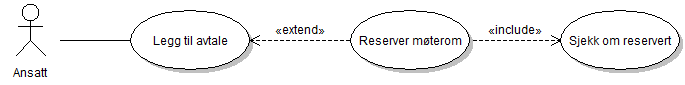
\includegraphics[width=400px]{ucs1.png}
\caption{Use Case-diagram for scenario 1}
\end{figure}

\subsection{Sekvensdiagram}
\begin{figure}[H]
\label{fig:sek1}
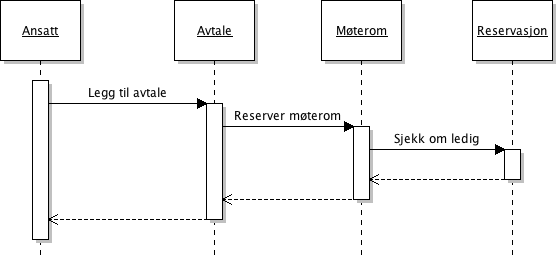
\includegraphics[width=400px]{sekvens1.png}
\caption{Use Case-diagram for scenario 1}
\end{figure}

\newpage
\section{Scenario 2}
\subsection{Use Case}
\begin{figure}[H]
\label{fig:uc2}
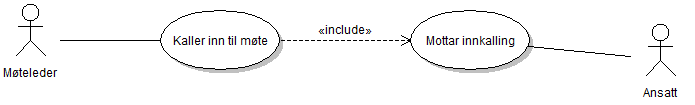
\includegraphics[width=400px]{ucs2.png}
\caption{Use Case-diagram for scenario 2}
\end{figure}

\subsection{Tekstlig Use Case}
\begin{table}[H]
\centering
\label{tab:tuc2}
\begin{tabular}{| l | L{4in} |}
\hline
Use Case & Scenario 2 \\
\hline
Aktør & Møteleder og inviterte ansatte \\
\hline
Trigger & Møteleder inviterer ansatte til et møte \\
\hline
Pre-betingelser & Møteleder har laget møtet \\
\hline
Post-betingelser & Ansatte er invitert til møtet, og mottar melding om dette når de logger seg på systemet. \\
\hline
Normal hendelsesflyt & 
\begin{minipage}{4in}
\vskip 4pt
\begin{itemize}
\item Møteleder opprettet møtet
\item Møteleder inviterer ansatte til møtet
\item Melding blir sendt til de inviterte, som de mottar neste gang de logger seg på
\end{itemize}
\vskip 4pt
\end{minipage}
 \\
\hline
Variasjoner & \\
\hline
Relatert informasjon & De inviterte medlemmene ser meldingen neste gang de logger seg på systemet. \\
\hline
\end{tabular}
\caption{Tekslig Use Case-diagrame}
\end{table}

\subsection{Sekvensdiagram}
\begin{figure}[H]
\label{fig:sek2}
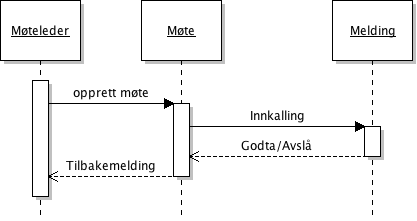
\includegraphics[width=400px]{sekvens2.png}
\caption{Use Case-diagram for scenario 2}
\end{figure}

\newpage
\section{Scenario 3}
\subsection{Use Case}
\begin{figure}[H]
\label{fig:uc3}
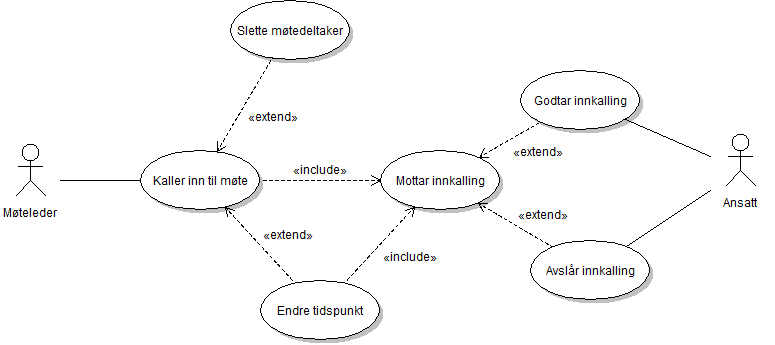
\includegraphics[width=400px]{ucs3.png}
\caption{Use Case-diagram for scenario 3}
\end{figure}

\subsection{Tekstlig Use Case}
\begin{table}[H]
\centering
\label{tab:tuc3}
\begin{tabular}{| l | L{4in} |}
\hline
Use Case & Scenario 3 \\
\hline
Aktør & Møteleder og inviterte ansatte \\
\hline
Trigger & Møteleder inkaller til møte \\
\hline
Pre-betingelser & Brukerene må være logget inn og invitert til samme møte. \\
\hline
Post-betingelser & Møtet blir satt hvor brukerene som har godtatt er invitert og de som har avlyst blir slettet fra møteinkallelsen. \\
\hline
Normal hendelsesflyt & 
\begin{minipage}{4in}
\vskip 4pt
\begin{itemize}
\item Møteleder inkaller til møte
\item Inviterte ansatte mottar møteinkallelse
\item Noen akspeterer møteinkalleslsen og noen avslår møteinkallelsen
\end{itemize}
\vskip 4pt
\end{minipage}
 \\
\hline
Variasjoner & 
\begin{minipage}{4in}
\vskip 4pt
\begin{itemize}
\item Møte blir planlagt på nytt
\item De som avslår møteinkallelsen blir slettet fra møteinkallelsen
\end{itemize}
\vskip 4pt
\end{minipage}
\\
\hline
Relatert informasjon & Alle ansatte som er invitert får beskjed om endringer som blir gjort i møteinkallelsen. \\
\hline
\end{tabular}
\caption{Tekslig Use Case-diagrame}
\end{table}

\subsection{Sekvensdiagram}
\begin{figure}[H]
\label{fig:sek3}
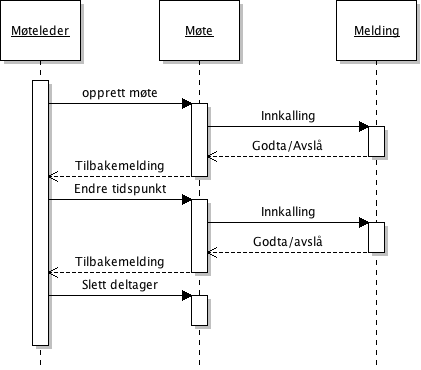
\includegraphics[width=400px]{sekvens3.png}
\caption{Use Case-diagram for scenario 3}
\end{figure}

\newpage
\section{Scenario 4}
\subsection{Tekstlig Use Case}
\begin{table}[H]
\centering
\label{tab:tuc4}
\begin{tabular}{| l | L{4in} |}
\hline
Use Case & Scenario 3 \\
\hline
Aktør & Møteleder og inviterte ansatte \\
\hline
Trigger & Møtelederen avlyser møtet \\
\hline
Pre-betingelser & Møtelederen har laget møtet og invitert andre ansatt. Noen ansatt må også ha godtat møtet. \\
\hline
Post-betingelser & Møten slettes og det gis bedskjed til de involverte ansatt. \\
\hline
Normal hendelsesflyt & 
\begin{minipage}{4in}
\vskip 4pt
\begin{itemize}
\item Møtelederen avlyser møtet.
\item Møtet blir slettet fra Møtelederens personlige kalender.
\item En melding blir sendt til alle inviterte medlemer.
\end{itemize}
\vskip 4pt
\end{minipage}
 \\
\hline
Variasjoner & \\
\hline
Relatert informasjon & De inviterte medlemer ser meldingen neste gang de logger seg på systemet. \\
\hline
\end{tabular}
\caption{Tekslig Use Case-diagrame}
\end{table}

\subsection{Sekvensdiagram}
\begin{figure}[H]
\label{fig:sek4}
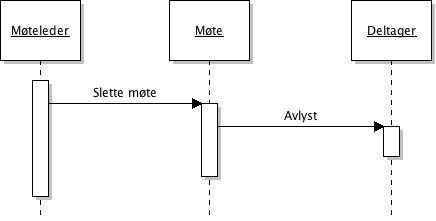
\includegraphics[width=400px]{sekvens4.png}
\caption{Use Case-diagram for scenario 4}
\end{figure}


\newpage
\listoftables

\newpage
\listoffigures

\newpage
\begin{thebibliography}{9}

\bibitem{fpkomp}
	Kompendium til fellesprosjektet,
	\emph{it's learning-gruppa til faget}
\end{thebibliography}

\end{document}
